\documentclass[a4paper]{article}

%use the english line for english reports
%usepackage[english]{babel}
\usepackage[portuguese]{babel}
\usepackage[utf8]{inputenc}
\usepackage{indentfirst}
\usepackage{graphicx}
\usepackage{verbatim}
\usepackage[margin=1.0in]{geometry}
\usepackage{listings}
\usepackage{color}

\definecolor{dkgreen}{rgb}{0,0.6,0}
\definecolor{gray}{rgb}{0.5,0.5,0.5}
\definecolor{mauve}{rgb}{0.58,0,0.82}

\begin{document}
\lstset{frame=none,
  language=C,
  aboveskip=3mm,
  belowskip=3mm,
  showstringspaces=false,
  columns=flexible,
  basicstyle={\small\ttfamily},
  numbers=none,
  numberstyle=\tiny\color{gray},
  keywordstyle=\color{blue},
  commentstyle=\color{dkgreen},
  stringstyle=\color{mauve},
  breaklines=true,
  breakatwhitespace=true,
  tabsize=3
}

\renewcommand{\figurename}{Fig.}

\setlength{\textwidth}{16cm}
\setlength{\textheight}{22cm}

\title{\Huge\textbf{Segundo Trabalho Laboratorial}\linebreak\linebreak\linebreak
\Large\textbf{Redes de Computadores}\linebreak\linebreak
\linebreak\linebreak

\includegraphics[scale=0.1]{feup-logo.png}\linebreak\linebreak
\linebreak\linebreak
\Large{Mestrado Integrado em Engenharia Informática} \linebreak\linebreak
\Large{Redes de computadores}\linebreak
}

\author{\textbf{Grupo:}\\
Carolina Centeio Jorge - up201403090 \\
João Fidalgo - up201303098 \\
Mónica Fernandes - up201404789 \\
Tiago Almeida - up201305665 \\
\linebreak\linebreak \\
 \\ Faculdade de Engenharia da Universidade do Porto \\ Rua Roberto Frias, s\/n, 4200-465 Porto, Portugal \linebreak\linebreak\linebreak
\linebreak\linebreak\vspace{1cm}}

\maketitle
\thispagestyle{empty}

%************************************************************************************************
%************************************************************************************************

\newpage

%Todas as figuras devem ser referidas no texto. %\ref{fig:codigoFigura}
%
%%Exemplo de código para inserção de figuras
%%\begin{figure}[h!]
%%\begin{center}
%%escolher entre uma das seguintes três linhas:
%%\includegraphics[height=20cm,width=15cm]{path relativo da imagem}
%%\includegraphics[scale=0.5]{path relativo da imagem}
%%\includegraphics{path relativo da imagem}
%%\caption{legenda da figura}
%%\label{fig:codigoFigura}
%%\end{center}
%%\end{figure}
%
%
%\textit{Para escrever em itálico}
%\textbf{Para escrever em negrito}
%Para escrever em letra normal
%``Para escrever texto entre aspas''
%
%Para fazer parágrafo, deixar uma linha em branco.
%
%Como fazer bullet points:
%\begin{itemize}
	%\item Item1
	%\item Item2
%\end{itemize}
%
%Como enumerar itens:
%\begin{enumerate}
	%\item Item 1
	%\item Item 2
%\end{enumerate}
%
%\begin{quote}``Isto é uma citação''\end{quote}


%%%%%%%%%%%%%%%%%%%%%%%%%%

\section{Summary}

Este projeto foi desenvolvido no âmbito da disciplina de Redes de Computadores (RCOM) do 3º ano do Mestrado Integrado em Engenharia Informática e Computadores da Faculdade de Engenharia da Universidade do Porto. Todos os conceitos usados neste trabalho foram lecionados tanto nas aulas teóricas como nas aulas teórico-práticas, dando especial atenção aos slides de \textit{Network}. O guia de laboratório foi também extremamente importante, pois continha todos os passos e comandos necessários para a realização deste projeto.

\section{Introdução}

Este projeto consiste em desenvolver uma aplicação através do protocolo FTP (descrito no RFC959) e realizar um conjunto de experiências com o objetivo de consolidar os conceitos lecionados nas aulas teóricas e perceber como configurar uma rede de computadores. Este projeto foi realizado em ambiente \textit{Linux} e desenvolvido em C.

A aplicação reduz-se a fazer download de um ficheiro, passado como argumento pelo utilizador, de um servidor FTP assim como também é possível especificar o \textit{username} e a \textit{password} se for necessário fazer \textit{login}, com a sintaxe descrita no RFC1738.

O propósito das experiências laboratoriais é dar a conhecer os comandos necessários para conseguir configurar uma redes de computadores. Esta segunda parte tem como objetivo configurar uma redes de computadores, todos ligados entre si através de duas VLANs diferentes configuradas num \textit{switch} assim como também configurar um \textit{router} comercial com \textit{NAT} e utilizar \textit{DNS} para a conversão de \textit{hostnames} em \textit{IP Addresses}.

O relatório tem uma secção dedicada a cada uma das duas partes deste projeto. O desenvolvimento da aplicação será explicado com grande detalhe na secção 3 e na secção 4 teremos subsecções para cada experiência realizada.

\section{Aplicação de Download}
Foi elaborado uma aplicação em C para fazer download de um ficheiro de um servidor FTP, usando ligações TCP. Esta aplicação implementa o protocolo FTP, como descrito em RFC959.

Esta aplicação é de um só argumento, sendo este um URL que segue a sintaxe descrita em RFC1738: \begin{verbatim} ftp://[<user>:>password>@]<host>/<url-path> \end{verbatim}
A aplicação começa por fazer parse desse URL, de forma a extrair a informação necessária para estabelecer a ligação TCP (user, password e host) e para, posteriormente, fazer download do ficheiro url-path. O user e password podem ser omitidos, sendo assumidos como “anonymous” e “mail@domain”, respetivamente.
Seguidamente, usando a função \textit{getip}, vamos buscar o ip correspondente ao endereço host escolhido pelo utilizador. Assim, já podemos abrir um socket TCP (chamemos-lhe A), usando a porta 21 e conectar ao servidor, através da função \textit{ftpConnect}. 
 
Se a ligação for bem sucedida, é enviado o user seguido da password em \textit{ftpLogin}. Se a resposta aos comandos de login for, também, positiva, tenta-se estabelecer o Passive Mode com a função \textit{ftpPasv}. Esta função, se não falhar, retorna a porta que vai servir para abrir o novo socket TCP (chamemos-lhe B). Neste novo socket, B, vai ser recebido o ficheiro que queremos fazer download, assim que, no primeiro socket aberto, A, enviarmos o comando “retr”, através da função \textit{ftpDownload}. A \textit{ftpDownload}, lê também o que vai sendo recebido no socket B e guarda num ficheiro, de forma a reproduzir inteiramente o ficheiro que queremos transferir.
No final, a ligação é terminada com o comando “quit” e são também fechados os sockets A e B e liberto o espaço em memória.

\section{Experiências Laboratoriais}
\subsection{Configuração de um IP de Rede}
Esta experiência permitiu-nos saber como distinguir os diferentes pacotes de dados assim como a sua funcionalidade e também como estabelecer ligados entre dois computadores.

Um dos pacotes de dados usados nesta experiência são os pacotes ARP (\textit{Address Resolution Protocol}). Este pacotes servem para obter o \textit{MAC Address} (endereço que identifica um computador na rede) de um determinado \textit{IP Address} (endereço que distingue um computador na rede). O computador onde é executado o comando \textit{ping} envia um comando para todos os computadores com que tem ligação e pergunta que computador tem o um determinado \textit{IP Address}. Este primeiro pacote envia o \textit{IP Address} do computador que se pretende descobrir o \textit{MAC Address} assim como o \textit{IP Address} do computador para o qual se deve responder. Um segundo pacote ARP é enviado como resposta com o \textit{IP Address} e o \textit{MAC Address} do computador em questão. Este mecanismo pode ser visto no anexo 7.1 nas linhas 22 e 23.

Outro tipo de pacotes são os ICMP (\textit{Internet Control Message Protocol}). Estes pacotes são gerados pelo comando ping e servem para enviar mensagens de erro ou de controlo para outros \textit{hosts} ou \textit{routers}. Quando um computador executa um comando ping, este envia um \textit{echo request} para o outro computador, com o seu \textit{IP Address} e o seu \textit{MAC Address} assim como o \textit{IP Address} e o \textit{MAC Address} do computador de destino. Por sua vez, o computador de destino envia uma resposta (\textit{echo reply}), com as mesmas informações. Este mecanismo pode ser confirmado no anexo 7.1 nas linhas 24 e 25.

Para descodificar estes pacotes é necessário analisar o \textit{IP Diagram Format} descrito nas aulas teóricas. O campo \textit{type of service} distingue se o pacote é ARP (0x0806) ou ICMP (0x0800). Isto pode ser visto no anexo 7.1 na segunda e terceira separação horizontal. O campo \textit{length} representa o tamanho total do \textit{datagram}. Este campo vem imediatamente a seguir ao campo \textit{type of service} e como podemos na zona mencionada acima este campo tem 0x0054 como valor, o que representa 84 bytes. 

O mecanismo de \textit{loopback} é um mecanismo que reenvia uma mensagem de volta para o computador que a envia. Isto permite detetar erros na transmissão de dados assim como problemas nos cabos de transmissão.

\subsection{Implementação de duas \textit{Virtual LANS} num switch}
Nesta experiência foi solicitada a criação de duas VLANS no switch. Para configurar uma VLAN temos de executar o comando “vlan x”, em que x corresponde ao número da vlan, na consola do switch. Depois de configurar as VLANS, foi necessário adicionar as respetivas portas no switch. Para adicionar a porta, basta selecioná-la e usar o comando “interface fastethernet 0/y”, em que y corresponde ao número da porta que queremos adicionar. Antes de adicionar a porta à VLAN com o comando “switchport access vlan x”, devemos alterar o seu modo com o comando “switchport mode access”.

Uma VLAN permite criar uma rede que é inacessível do interior para o exterior e vice versa. Assim, depois da observação dos logs da experiência 2, podemos concluir que existem 2 broadcast domains, um em cada VLAN. Podemos verificar, a partir do anexo 7.2, que quando o tux1 fez um pedido broadcast apenas o tux dessa mesma VLAN (Tux 4) recebeu o request. Embora os tuxs estejam todos no mesmo switch, os pacotes só eram recebidos por tuxs dentro da mesma VLAN.

\subsection{Configurar um \textit{router} em Linux}
Esta experiência consiste em "ligar" as duas VLANs criada na experiência anterior, fazendo com o Tux4 de comporte como um \textit{router}.

Nesta experiência começamos por configurar a eth0 e eth1 do Tux4 para que cada uma pertencesse a uma VLAN diferente. Para isso basta configurar os IPs de cada interface de forma a corresponder com a VLAN repetiva, utilizando o comando \textit{ifconfig ethX [IP Address]}, sendo X 0 ou 1. De seguida adicionámos rotas ao Tux1 e ao Tux2 de forma a que seja possível enviar pacotes entre um e outro. Para isso utilizamos o comando \textit{route add -net [IP da subrede] gw [IP Address do gateway]}, em que neste caso o gateway é o Tux4. Sendo, um exemplo deste comando seria \textit{route add -net 172.16.30.0/24 gw 172.16.30.254}. Nesta fase da experiência, o Tux1 e o Tux2 devem ter duas rotas, uma criada automaticamente quando é atribuído um IP à interface \textit{ethernet} e outra que os liga mutuamente através do Tux4. O Tux4 deve ter apenas as duas rotas que são criadas automaticamente para cada um das suas interfaces \textit{ethernet}.

A \textit{forwarding table} guarda informações sobre a rede de destino, o \textit{gateway} que faz a ligação a essa rede, a máscara dessa rede e a interface associada.



\subsection{Configurar um router comercial e implementar NAT}

O objetivo desta experiência era configurar um \textit{router} comercial com NAT (\textit{Network Address Resolution}) e perceber a sua funcionalidade.

A primeira parte desta experiência consiste em configurar o \textit{router} sem NAT. Para isso, configuramos cada uma das interfaces \textit{gigabitethternet} com os seguintes comandos:
\begin{itemize}
	\item \textit{ip address [ip address] [mascara de rede]}
	\item \textit{no shutdown}
\end{itemize}
e configurmos as rotas com o comando \textit{ip route [rede de destino] [mascara de rede] [gateway IP]}. Com isto, foi possível configurar cada uma das interfaces de forma a que cada computador na rede privada tivesse acesso ao \textit{router} comercial. Neste momento da experiência percebemos que os pacotes do comando \textit{ping} entre o computador 2 e o computador 1 percorriam o seguinte caminho tux2 -\textgreater tux4 -\textgreater tux1. Isto acontecia, porque o tux2 tinha uma route para a outra VLAN apartir do tux4. Removendo essa rota, o caminho passa a ser tux2-\textgreater \textit{router} -\textgreater tux4 -\textgreater tux1. Sem \textit{redirects}, este caminho é percorrido todas as vezes que é enviado um pacote, no entanto, se ativarmos os \textit{redirects} este caminho é apenas percorrido uma vez e os seguintes já percorrem a rota tux2 -\textgreater tux4 -\textgreater tux1.

A segunda parte consiste em adicionar NAT ao router para que esta rede privada possa ter acesso a uma rede na \textit{internet}. A NAT é uma funcionalidade que permite que o endereço de um computador numa rede privada seja traduzido num \textit{IP Address} válido na \textit{internet}. A NAT recebe o \textit{IP Address} interno e a porta local do computador e gera um endereço de 16 bits usando uma tabela hash, sendo este endereço então escrito no campo da porta de origem. Com este mecanismo, o \textit{router} é capaz de enviar pacotes de dados para o exterior da rede privada a partir de um \textit{IP Address} global e do \textit{IP Address} gerado com o mecanismo descrito anteriormente e quando recebe uma resposta, consegue descobrir qual será o computador que terá de receber a resposta.

Para configure a NAT no \textit{router} basta adicionar \textit{ip nar inside} à interface que está ligada à rede privada e \textit{ip nat outside} à interface ligado à rede externa.
\subsection{DNS}
Com esta experiência percebemos como configurar o servidor \textit{DNS} assim como o seu papel e a sua importância nas redes de computadores.

De uma forma breve, o servidor \textit{DNS} serve para traduzir um \textit{hostname} (www.google.com) num \textit{IP Address} (194.210.238.155) atrás do \textit{DNS Resolver}.

A configuração do servidor \textit{DNS} trata-se apenas da edição do ficheiro /etc/resolv.conf, adicionando uma linha a especificar o \textit{search} (netlab.fe.up.pt) e o \textit{nameserver} (172.16.1.1).

O primeiro pacote é enviado ao servidor \textit{DNS} com o nome do \textit{host} que por sua vez é passado como argumento ao \textit{resolver} e este devolve o \textit{IP Address} ligado a esse \textit{hostname}. O segundo pacote envia um \textit{IP Address} e espera pelo respetivo \textit{hostname}. Este último mecanismo é chamado \textit{reverse DNS lookup}.

\subsection{Ligações TCP}
Esta experiência pretende testar e analisar resultados relativos à aplicação FTP que elaborámos. A aplicação, como analisado anteriormente, estabelece duas ligações TCP. A primeira, através do socket a que chamámos A, onde é transportada a informação de controlo FTP através do comando “pasv”.

A ligação TCP divide-se em três fases e em todas é possível analisar um conjunto de parâmetros como a source port e a destination port (as mesmas durante toda a aplicação), o ARQ (por flag, neste caso ACK ou SYN), o sequence number, o Acknowledgment number e o window size. O mecanismo de ARQ em TCP funciona como Selective Repeat ARQ: o emissor envia o número de frames equivalente ao window size sem sem esperar por um ACK. Este window size é determinado pelo recetor, enquanto que a congestion window é determinada pelo emissor e não é visível nos logs. O recetor pode rejeitar frames individualmente, que posteriormente serão reenviados. 

\begin{figure}[!ht]
\centering
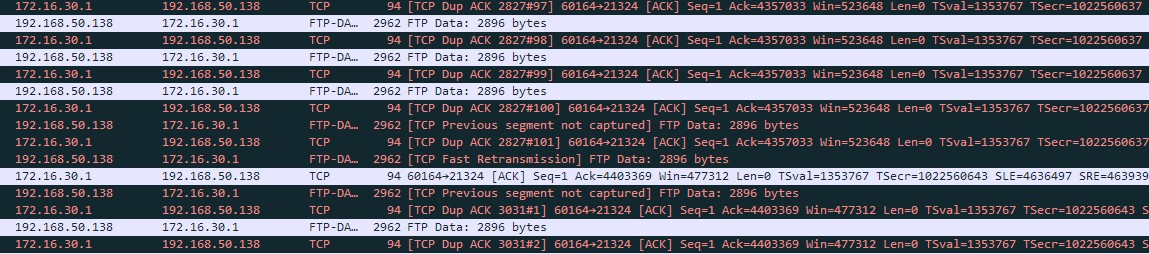
\includegraphics[scale=0.35]{retrans_tcp.jpg} 
\end{figure}

Aqui, o parâmetro ACK terá sido menor que o último byte enviado pelo emissor. O recetor detetou a falha na sequência de números e gerou um ACK duplicado para pacote subsequente recebido nessa ligação, até que o pacote em falta tenha sido recebido com sucesso.

As três fases são, então:

- Estabelecimento de ligação: desde a abertura do socket, ao processamento dos dados de user e password 

\begin{figure}[!ht]
\centering
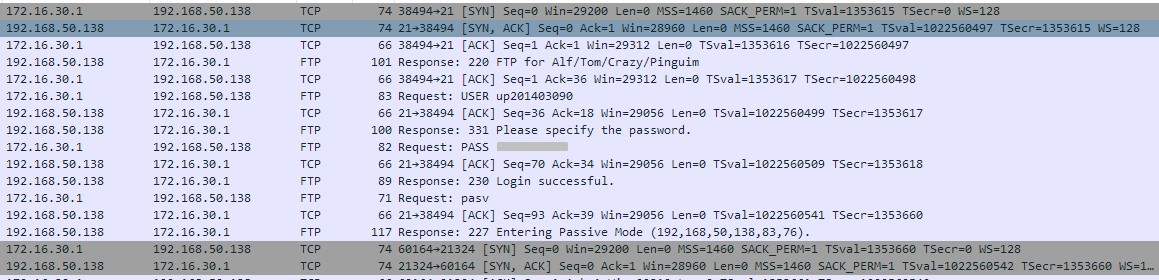
\includegraphics[scale=0.35]{connection_tcp.jpg}
\end{figure}

- Transferência de dados: desde o envio do comando “retr” até ao final da transferência do ficheiro em causa. 

\begin{figure}[!ht]
\centering
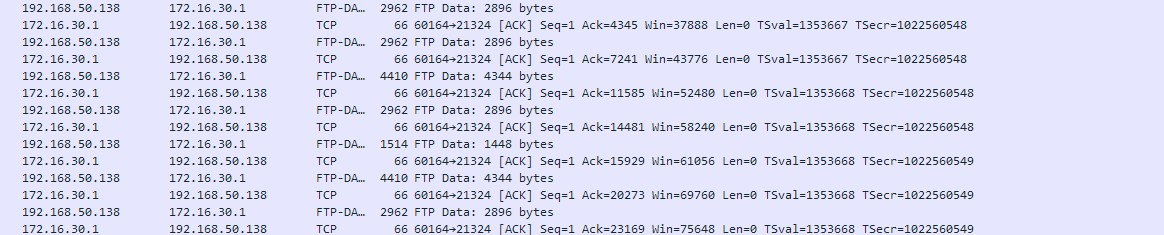
\includegraphics[scale=0.35]{trans_tcp.jpg}
\end{figure}

- Término de ligação: o envio do quit seguido da receção do “Goodbye” termina a ligação 

\begin{figure}[!ht]
\centering
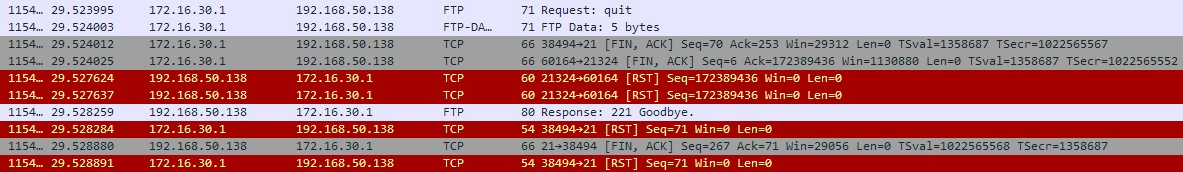
\includegraphics[scale=0.35]{quit_tcp.jpg}
\end{figure}

É notável que o número de pacotes transferidos com sucesso, por segundo, diminui quando outra ligação TCP é iniciada. Nesta segunda, notamos também um aumento significativo quando a primeira transferência acaba. Tentámos juntar num só gráfico o que acabámos de explicar: 

\begin{figure}[!ht]
\centering
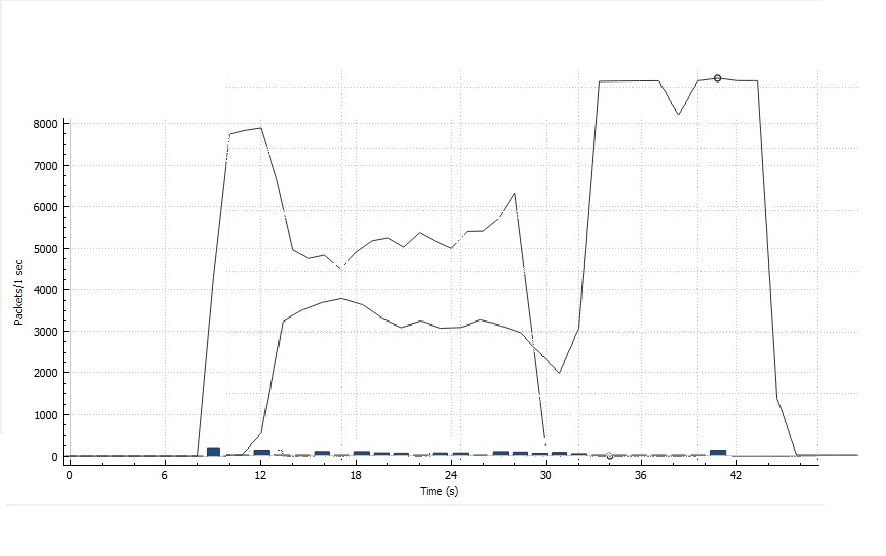
\includegraphics[scale=0.35]{tuxexp6.jpg}
\end{figure}

\section{Conclusão}

Todas as experiências foram realizadas com sucesso e com elas fomos capazes de aplicar os conceitos dados nas aulas teóricas. 

Conclui-se que a configuração de um rede de pequena dimensão é um problema sem grande complexidade, no entanto para a configuração de uma rede de mais dimensão é necessário aprofundar certos conceitos e aprender novos que não foram lecionados nesta unidade curricular.

\textbf{Falar das conclusões da experiência 6, alterações no tráfego quando duas aplicações estão a ser corridas ao mesmo tempo, etc...}.

\section{Contribuições}

Sumário, experiência 4 e 5 foram feitos pelo Tiago Almeida.

Introdução, experiência 1 e conclusão foram feitos pela Mónica Fernandes.

Aplicação FTP e experiência 6 foram feitos pela Carolina Centeio.

Experiência 2 e 3 foram feitas pelo João Fidalgo.

\newpage
\section{Anexos}
\subsection{Experiência 1}

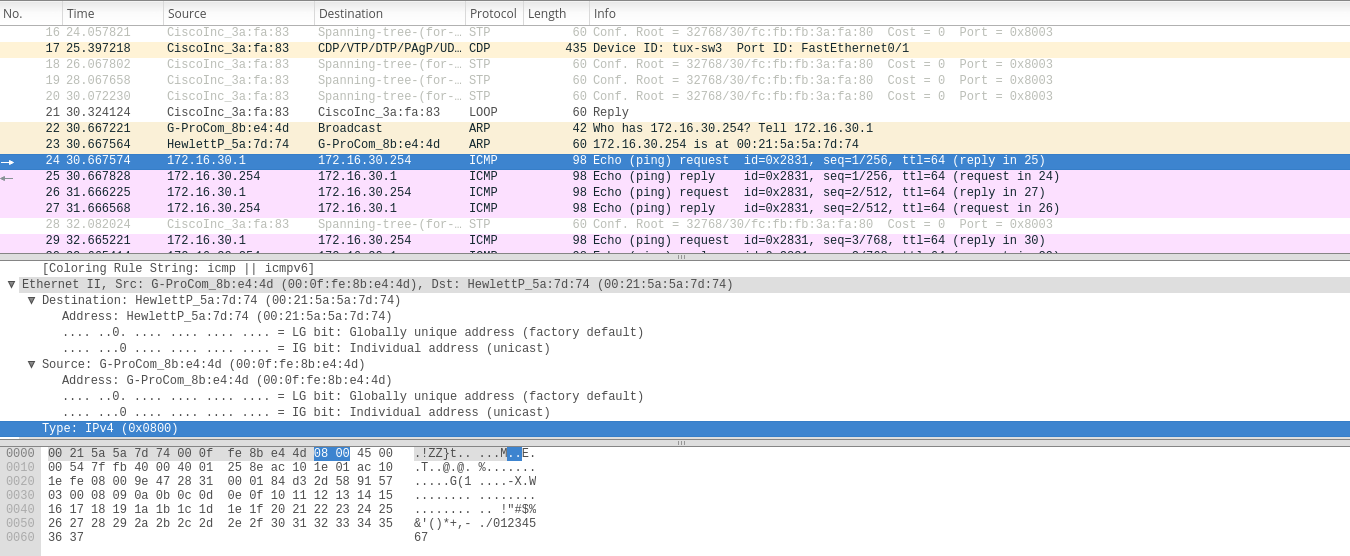
\includegraphics[scale=0.35]{Exp1.png}

\subsection{Experiência 2}

\subsubsection{Tux 1}
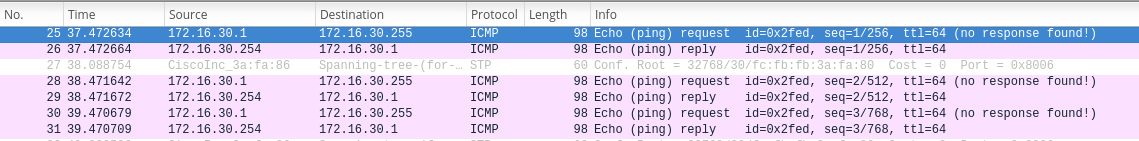
\includegraphics[scale=0.35]{Exp2-tux1.png}

\subsubsection{Tux 2}
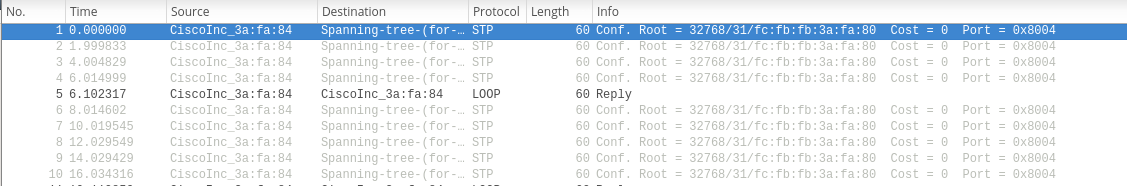
\includegraphics[scale=0.35]{Exp2-tux2.png}

\subsubsection{Tux 4}
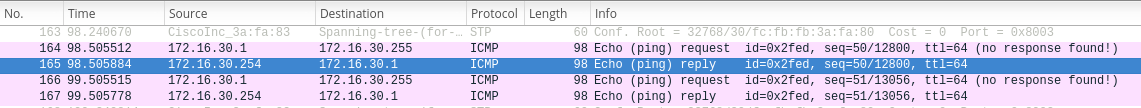
\includegraphics[scale=0.35]{Exp2-tux4.png}

\subsection{Experiência 3}
\subsubsection{Tux 1 -\textgreater 2}

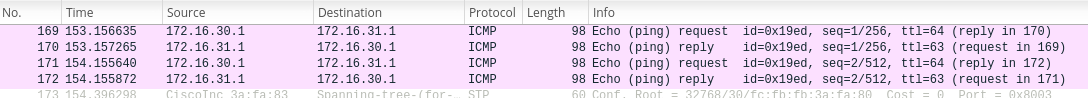
\includegraphics[scale=0.35]{Exp3-Tux1-2.png}

\subsubsection{Tux 1 -\textgreater 4}

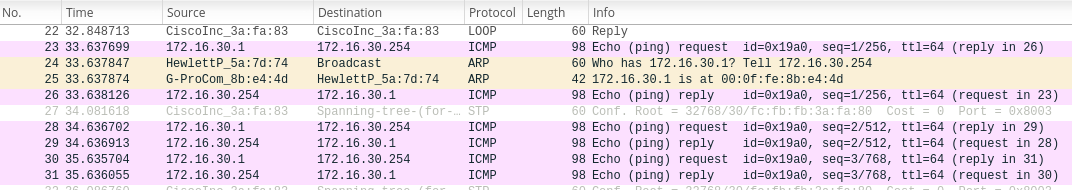
\includegraphics[scale=0.35]{Exp3-Tux1-4.png}

\subsubsection{Tux 4 - Eth0}

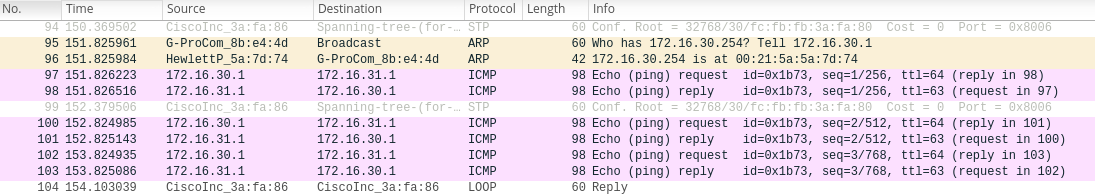
\includegraphics[scale=0.35]{Exp3-Tux4-eth0.png}

\subsubsection{Tux 4 - Eth1}

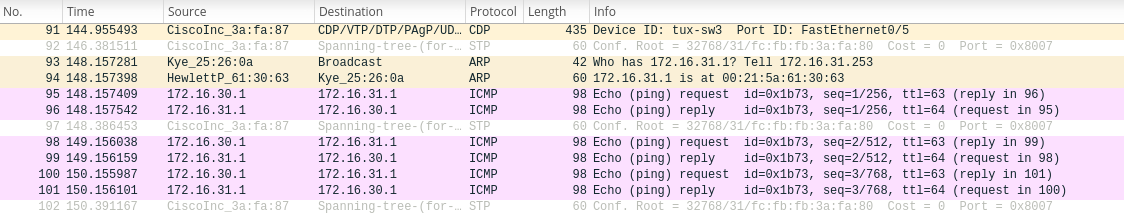
\includegraphics[scale=0.35]{Exp3-Tux4-eth1.png}

\subsection{Experiência 4}
\subsubsection{Passo 4 - Sem Redirect}

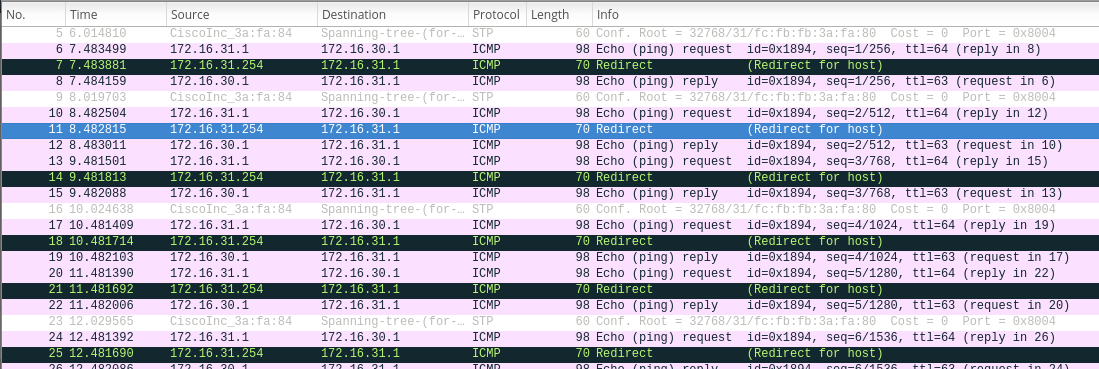
\includegraphics[scale=0.35]{Exp4-4-withoutRedirect.png}

\subsubsection{Passo 4 - Com Redirect}

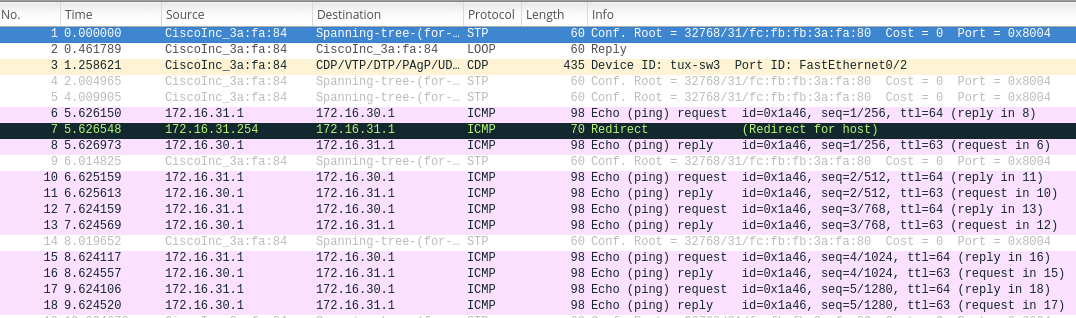
\includegraphics[scale=0.35]{Exp4-4-withRedirect.png}

\subsubsection{Passo 5 - NAT}

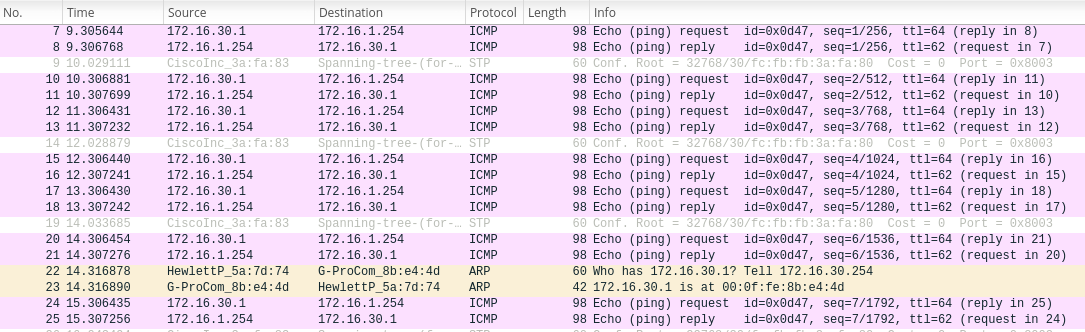
\includegraphics[scale=0.35]{Exp4-5-NAT.png}

\subsection{Experiência 5}

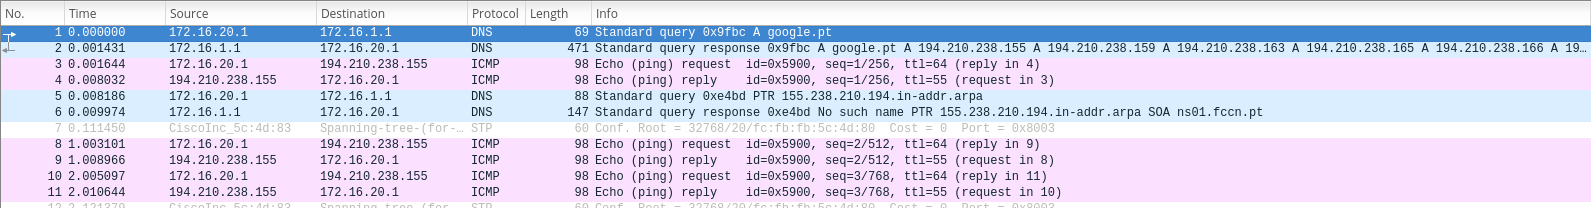
\includegraphics[scale=0.30]{Exp5-DNS.png}

\newpage

\section{Código fonte da aplicação FTP}
\begin{verbatim}
#include <sys/types.h>
#include <sys/socket.h>
#include <netdb.h>
#include <stdio.h>
#include <stdlib.h>
#include <unistd.h>
#include <errno.h>
#include <string.h>
#include <netinet/in.h>
#include <arpa/inet.h>
#include <fcntl.h>

#define MESSAGE_SIZE 200

int getip(char *host, char *hostaddr)
{
	struct hostent *h = malloc(sizeof(struct hostent));

/*
struct hostent {
	char    *h_name;	Official name of the host.
    char    **h_aliases;	A NULL-terminated array of alternate names for the host.
	int     h_addrtype;	The type of address being returned; usually AF_INET.
    int     h_length;	The length of the address in bytes.
	char    **h_addr_list;	A zero-terminated array of network addresses for the host.
	Host addresses are in Network Byte Order.
};
#define h_addr h_addr_list[0]	The first address in h_addr_list.
*/
    if ((h=gethostbyname(host)) == NULL) {
        herror("gethostbyname");
        return -1;
    }

    printf("Host name  : %s\n", h->h_name);
    printf("IP Address : %s\n",inet_ntoa(*((struct in_addr *)h->h_addr)));
    strcpy(hostaddr, inet_ntoa(*((struct in_addr *)h->h_addr)));
	printf("Free h\n");
    return 0;
}

int ftpLogin(int socketfd, char* user, char* pass){
  	printf("Login\n");
	char reply[MESSAGE_SIZE] = "", *usercmd = malloc(sizeof(char) * MESSAGE_SIZE), *passcmd = malloc(sizeof(char) * MESSAGE_SIZE);

	read(socketfd, reply, MESSAGE_SIZE);

	sprintf(usercmd, "USER %s\n", user);
  	printf("%s\n", usercmd);
	write(socketfd, usercmd, strlen(usercmd));
	read(socketfd, reply, MESSAGE_SIZE);
	printf("%s\n", reply);

	bzero(reply, strlen(reply));

	sprintf(passcmd, "PASS %s\n", pass);
  	printf("%s\n", passcmd);
	write(socketfd, passcmd, strlen(passcmd));
	read(socketfd, reply, MESSAGE_SIZE);

	printf("%s\n", reply);

	if (reply[0] == '2' && reply[1] == '3' && reply[2]== '0'){
		free(usercmd);
		free(passcmd);
		return 0; //SUCCESS
	}

	free(usercmd);
	free(passcmd);
	return -1;

}

int ftpPasv(int shost, char* host, unsigned int *port){
	char reply[MESSAGE_SIZE] = "", *command =  "pasv\n";
  	int h1, h2, h3, h4, h5, h6;

  	bzero(reply, strlen(reply));

	write(shost, command, strlen(command));
	read(shost, reply, MESSAGE_SIZE);

  	if(sscanf(reply, "227 Entering Passive Mode (%d,%d,%d,%d,%d,%d)\n", &h1, &h2, &h3, &h4, &h5, &h6) != 6){
    	printf("Answer does not match for Passive Mode:\n --> %s \n", reply);
    	return -1;
  	}

	sprintf(host, "%d.%d.%d.%d", h1, h2, h3, h4);
	*port = h5*256 + h6;

	return 0;
}

int ftpDownload(int socketfd, int shost, char* filename, char* path) {
	char reply[MESSAGE_SIZE] = "", *retrcmd = malloc(sizeof(char) * MESSAGE_SIZE);

	bzero(reply, strlen(reply));
	sprintf(retrcmd, "retr %s\n", path);
	printf("Path: %s\nFilename. %s\n", path, filename);

	write(socketfd, retrcmd, strlen(retrcmd));
	read(socketfd, reply, MESSAGE_SIZE);
	printf("Reply: %s\n", reply);


  if (reply[0] == '1' && reply[1] == '5' && reply[2]== '0') {

    int fd =  open(filename, O_WRONLY | O_CREAT, 0777), nbytes = 0, counter = 0;
    char* trans = malloc(sizeof(char) * MESSAGE_SIZE);

    while((nbytes = read(shost, trans, MESSAGE_SIZE)) != 0) {
		if(!(counter % 1000))
			printf(".");
		fflush(stdout);
		counter++;	      
		write(fd, trans, nbytes);
	}

	printf("\n");

    close(fd);

    bzero(reply, strlen(reply));
    read(socketfd, reply, MESSAGE_SIZE);

    if (reply[0] == '2'){

		printf("Download succeeded\n");
		free(trans);
		free(retrcmd);
		return 0; //SUCCESS
	}

	printf("Download failed\n");

  }

	free(retrcmd);
	return -1;

}

int parseURL(char * url, char * host, char * path, char * user, char * pass, char* filename){

	int ret = sscanf(url, "ftp://%[^:]:%[^@]@%[^/]/%s\n", user, pass, host, path);
	if(ret != 4){
		ret = sscanf(url, "ftp://%[^/]/%s\n", host, path);
		if (ret != 2) {
			return -1;
      	}
      	strcpy(user, "anonymous");
      	strcpy(pass, "mail@domain");
    } //not success

	char * last = strrchr(path,'/');
	strcpy(filename, last+1);

	printf("Filename: %s\n", filename);
	return 0; //success
}

int ftpConnect(char* server_ip, const unsigned int port){
	//connect socket
	struct	sockaddr_in server_addr;
	int sockfd;

	/*server address handling*/
	bzero((char*)&server_addr, sizeof(server_addr));
	server_addr.sin_family = AF_INET;
	server_addr.sin_addr.s_addr = inet_addr(server_ip);	/*32 bit Internet address network byte ordered*/
	server_addr.sin_port = htons(port);		/*server TCP port must be network byte ordered */
	/*open an TCP socket*/
	if ((sockfd = socket(AF_INET,SOCK_STREAM,0)) < 0) {
		perror("socket()");
		return -1;
	}

	/*connect to the server*/
  if(connect(sockfd, (struct sockaddr *)&server_addr, sizeof(server_addr)) < 0){	
        	perror("connect()");
			return -1;
	}

	return sockfd;
}

int main(int argc, char **argv){

	char host[MESSAGE_SIZE] = "";
	char path[MESSAGE_SIZE] = ""; 
	char user[MESSAGE_SIZE] = "";
	char pass[MESSAGE_SIZE] = "";
	char filename[MESSAGE_SIZE] = "";



	if(argc != 2){
		printf("usage: download ftp://[<user>:<password>@]<host>/<url-path> \n");
		return -1;
	}
  	printf("Going to parse\n");

	if(parseURL(argv[1], host, path, user, pass, filename) == -1){
		printf("url does not match ftp://[<user>:<password>@]<host>/<url-path> \n");
		return -1;
	}
  	printf("Finished parse\n");

	
	char* hostaddr = malloc(sizeof(char) * MESSAGE_SIZE);

	if(getip(host, hostaddr) != 0){
		printf("Failed getting ip\n");
		free(hostaddr);		
		return -1;
	}

	unsigned int port = 21, sport;

	printf("Starting connection...\n");
	printf("%s\n", hostaddr);

	int sockfd = ftpConnect(hostaddr, port);

	printf("ftpconnect done\n");

	if(sockfd == -1){
		free(hostaddr);
		printf("Connection failed\n");
		return -1;
	}

	//login
	if(ftpLogin(sockfd, user, pass) != 0){
	free(hostaddr);
	close(sockfd);
    printf("Login failed\n");
    return -1;
  }

	printf("Login succeeded\n");

	//passv - calcular a porta
	char *shost = malloc(sizeof(char)*MESSAGE_SIZE);
	if(ftpPasv(sockfd, shost, &sport) != 0){
		printf("Passive Mode Failed\n");
		free(hostaddr);
		free(shost);
		close(sockfd);
		return -1;
  }


	printf("Passive Mode Established\n");
	int sockhost = ftpConnect(shost, sport);
	if(sockhost == -1){
		printf("Connection failed\n");
		free(hostaddr);
		free(shost);
		close(sockfd);
		return -1;
	}
	//download
	if(ftpDownload(sockfd, sockhost, filename, path) != 0){
		free(hostaddr);
		free(shost);
		close(sockfd);
		close(sockhost);

    printf("Download failed\n");
    return -1;
  }
  printf("Download finished\n");

	char* quit = "quit\n";
	write(sockfd, quit, strlen(quit));
	write(sockhost, quit, strlen(quit));

	free(hostaddr);
	free(shost);
	close(sockfd);
	close(sockhost);

	return 0;

}
\end{verbatim}

\end{document}
